\subsection{Communication Test Results}
\label{sec:communication_results}
\newrevision{The historical eight-byte experiment is separate from the current version-5, 34-byte result demonstration in Section~\ref{sec:communication_protocol}. The supplied \texttt{Com Logs.csv} contains 50 runs requesting 1,000 packets each. The team confirmed the test settings and packet layout in Tables~\ref{tab:communication_setup} and~\ref{tab:communication_payload}. Tests included different distances and did not have full line of sight: objects and reflective materials were present around the test area. Their individual effects were not isolated. The furthest successful communication distance reached was 350 m with the current hardware and spring antennas. This is the maximum distance reached during these tests, rather than an established maximum radio range. Individual CSV rows are not mapped to distance, and the test date remains unreported.}

\begin{table}[htbp]
\centering
\caption{\newrevision{Team-confirmed communication experiment configuration.}}
\label{tab:communication_setup}
\begin{tabular}{p{0.40\textwidth}p{0.50\textwidth}}
\toprule
Setting & Value \\
\midrule
Radio / frequency & SX1278 / 433 MHz \\
Spreading factor & SF7 \\
Bandwidth & 125 kHz \\
Coding rate & 4/5 \\
Configured TX power & 10 dBm \\
Antennas & 433 MHz spring antennas \\
Test conditions & Partial obstruction; objects and reflective materials nearby \\
\newrevision{DATA / application} & \newrevision{8 bytes / 6 bytes, synthetic records} \\
\bottomrule
\end{tabular}
\end{table}

\begin{table}[htbp]
\centering
\caption{\newrevision{Historical eight-byte DATA packet: two-byte sequence and six-byte application record.}}
\label{tab:communication_payload}
\begin{tabular}{p{0.16\textwidth}p{0.74\textwidth}}
\toprule
Byte offsets & Contents \\
\midrule
0--1 & Sequence number: unsigned 16-bit integer, little-endian \\
2 & Node ID \\
3 & Day (five bits) and battery code (three bits) \\
4--7 & Synthetic probability: \texttt{(sequence \% 101) / 100.0f}, float32, little-endian \\
\bottomrule
\end{tabular}
\end{table}

\newrevision{The probability field is generated from the sequence number; it is not a classifier prediction. These packets contain neither MFCC coefficients nor measured RPW detection results. DATA byte 3 holds day in bits 7--3 and battery in bits 2--0. The battery code is $\operatorname{round}(7\,\operatorname{clamp}(P,0,100)/100)$ for input percentage $P$; codes are 0--7. Day is 1--31. The experimental defaults (node 1, day 15, simulated battery 80\%, code 6) are not measured calendar/battery telemetry. The eight DATA bytes comprise two sequence bytes and six application bytes; PHY and control-message overhead are additional.}
\FloatBarrier

\begin{table}[htbp]
\centering
\caption{\newrevision{Summary of 50 historical eight-byte communication runs.}}
\label{tab:communication_results}
\begin{tabular}{p{0.51\textwidth}p{0.39\textwidth}}
\toprule
Measure & Result \\
\midrule
Original packets requested & 50,000 \\
Furthest distance reached (team-reported) & 350 m, current hardware and antenna \\
Initial unique packets received & 49,710 (99.42\%) \\
Initial missing packets & 290 (0.58\%) \\
Additional ARQ DATA transmissions & 290 \\
Recovered packets & 290 \\
Final unique packets received & 50,000 (100\%) \\
Final missing / reported duplicates & 0 / 0 \\
Initial loss per run & 0--2.2\% \\
Observation duration & Mean 113.147 s; range 110.483--119.138 s \\
Delivered records per second & Mean 8.869; range 8.418--9.080 \\
Logged application goodput & Mean 425.704 bit/s; range 404.040--435.853 \\
Logged DATA goodput & Mean 567.606 bit/s; range 538.721--581.137 \\
Mean send-call duration & 36.871 ms; run means 36.865--36.875 ms \\
RSSI run averages & $-103.70$ to $-52.57$ dBm \\
SNR run averages & 3.69--9.87 dB \\
\bottomrule
\end{tabular}
\end{table}

\newrevision{Automatic repeat request (ARQ) recovered all initial misses. Each run completed 1,000 original transmissions, with no locally failed/skipped records reported. Additional DATA retransmissions equal 0.58\% of original packets; this excludes control-message and acknowledgement overhead. Final delivery was 100\% in every recorded run, rather than a guarantee for other conditions.}

\begin{figure}[htbp]
\centering
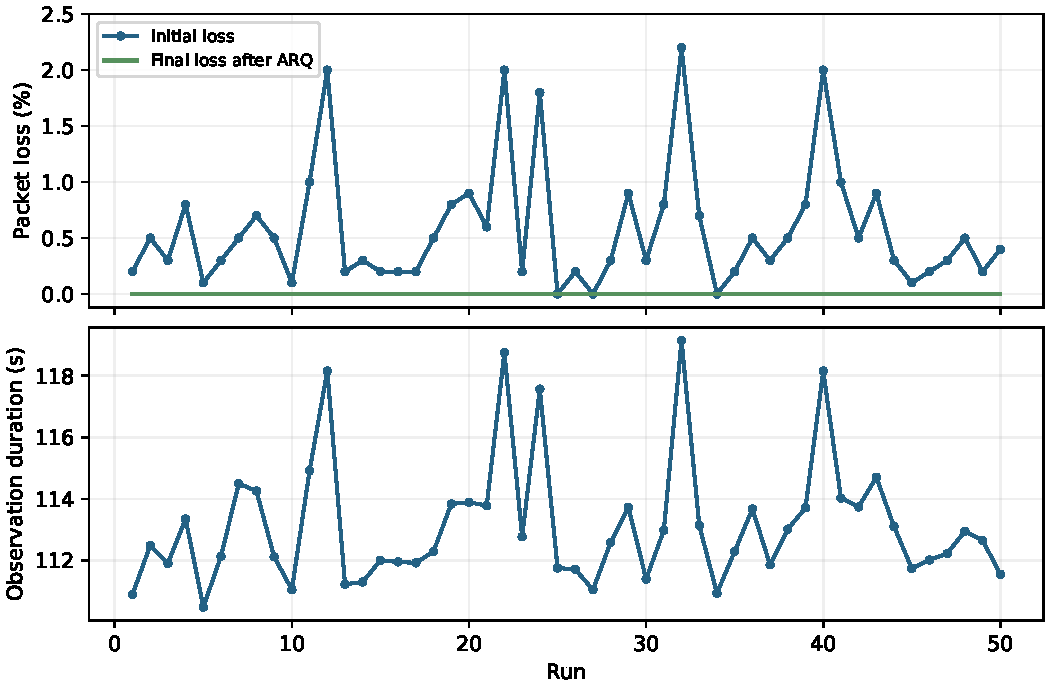
\includegraphics[width=\textwidth]{figures/communication_runs.pdf}
\caption{\newrevision{Initial/final loss and observation duration in CSV row order across tests that included different distances. Distances are not assigned to individual rows, so the horizontal axis is run number.}}
\end{figure}

\newrevision{DATA send calls total approximately 36.9--37.7 s per run, while receiver observation averages approximately 113 s. Send-call duration is not end-to-end latency. The historical Control-Fix scheduler reserves 125 eight-record windows of 872 ms (109 s) plus a fixed 10 s retry allowance, giving a 119 s single-session assignment. The reported timing is consistent with that configuration; the 50-run binary/build provenance still needs confirmation. This is unrelated to the current 1,099 ms per-node slot. Overrun compares actual sender slot elapsed with the fixed assignment on the sender clock, excluding START setup and final END reporting. Receiver START-to-first-END observation has different boundaries: a 119.138 s observation does not establish overrun when the corresponding sender schedule is about 118.8 s. Runs continue after the assignment for measurement and must report the sender overrun flag.}

\newrevision{Logger definitions are available from the experimental source. For $U$ final unique valid records and actual sender slot elapsed $T$ seconds, delivered records/s is $U/T$, application goodput is $48U/T$ bit/s and DATA goodput is $64U/T$ bit/s. Retries and control delays contribute to $T$ but their bytes are not additional useful delivery. The 48:64 ratio agrees with the six- versus eight-byte definitions. These are neither 34-byte-demo nor compressed-MFCC throughput measurements. Means are arithmetic run averages across the combined tests; RSSI/SNR ranges describe run averages, not instantaneous extremes. Without a run-to-distance mapping, these aggregate delivery and throughput values cannot be assigned specifically to 350 m or used to plot performance versus distance. These logs demonstrate packet reception and recovery but do not establish Wi-Fi/cloud forwarding or classifier and codec correctness. The power experiment also used eight-byte packets. Its 42 s run duration differs from the communication-log observation durations, so combining the energy and delivery results still requires matched timing and measurement boundaries. Per-run distances, radio airtime, and end-to-end latency remain pending.}
\FloatBarrier
